\documentclass{article}
\linespread{1.3}
\usepackage[margin=50pt]{geometry}
\usepackage{amsmath, amsthm, amssymb, amsthm, tikz, fancyhdr, graphicx, subfig}
\pagestyle{fancy}
\renewcommand{\headrulewidth}{0pt}
\newcommand{\changefont}{\fontsize{15}{15}\selectfont}

\newcommand{\field}[1]{\mathbb{#1}}
\newcommand{\1}{\mathbf{1}}
\newcommand{\E}{\mathbb{E}} 
\renewcommand{\P}{\mathbb{P}}
\newcommand{\R}{\field{R}} % real domain
% \newcommand{\C}{\field{C}} % complex domain
\newcommand{\F}{\field{F}} % functional domain

\newcommand{\T}{^{\textrm T}} % transpose

\def\diag{\text{diag}}

%% operator in linear algebra, functional analysis
\newcommand{\inner}[2]{#1\cdot #2}
\newcommand{\norm}[1]{\left\|#1\right\|}
\newcommand{\twonorm}[1]{\|#1\|_2^2}
% operator in functios, maps such as M: domain1 --> domain 2
\newcommand{\Map}[1]{\mathcal{#1}}
\renewcommand{\theenumi}{\alph{enumi}} 

\newcommand{\Perp}{\perp \! \! \! \perp}

\newcommand\independent{\protect\mathpalette{\protect\independenT}{\perp}}
\def\independenT#1#2{\mathrel{\rlap{$#1#2$}\mkern2mu{#1#2}}}
\newcommand{\vct}[1]{\boldsymbol{#1}} % vector
\newcommand{\mat}[1]{\boldsymbol{#1}} % matrix
\newcommand{\cst}[1]{\mathsf{#1}} % constant
\newcommand{\ProbOpr}[1]{\mathbb{#1}}
\newcommand{\points}[1]{\small\textcolor{magenta}{\emph{[#1 points]}} \normalsize}
\date{{}}

\fancypagestyle{firstpageheader}
{
  \fancyhead[R]{\changefont Michael Huang \\ CSE 446 \\ Homework 3}
}

\begin{document}

\thispagestyle{firstpageheader}

\section*{Collaborators}
{\Large 
Jimmy Guo, Neil Kagalwala, Andrew Wang
}
\section*{A.1}
{\Large 

\subsection*{a.}

If the RBF kernel underfits the training set, we should decrease the bandwidth $\sigma$. Underfitting indicates a smoother fit and lower variance, so we want to decrease $\sigma$ so that we fit the training points more tightly.
% more narrow bumps and fits data more tightly

\subsection*{b.}

True. With a non-convex loss function, gradient descent is not guaranteed to go all the way towards the global minimum, and could even stagnate or increase.
% Could increase?

\subsection*{c.}

False. When training a deep neural network, we should initialize weights to random values. One reason for this is that with any equal weight initialization, all nodes will have the same gradient, so the nodes will end up all following the same pattern and an ineffective model overall.

\subsection*{d.}

True. We try to use non-linear activation functions in order to introduce non-linearity into the network. If we only had linear activation functions, then the model would essentially just output a linear function, since no matter how many layers, all the linear functions would naturally sum together, and lead to what is essentially basic logistic regression.

\subsection*{e.}

True. The time complexity for the forward pass is lower than that of the backward pass in the backpropagation algorithm. backpropagation first requires calculating values via forward-propagation itself, and then performing error calculation and gradient descent to update these values, which can be prohibitively slow compared to just the forward-propagation step.

}

\section*{A.2}
{\Large

We aim to show that $K(x, x') = e^{-\frac{(x-x')^2}{2}}$ is a kernel function for the defined feature map, or that $\phi (x) \cdot \phi (x') = e^{-\frac{(x-x')^2}{2}}$. \\ \\
We are given that the $i$th component of the vector $\phi(x)$ is defined as $\frac{1}{\sqrt{i!}} e^{-x^2/2} x^i$, and we can naturally express $\phi(x')$ as  $\frac{1}{\sqrt{i!}} e^{-(x')^2 / 2} (x')^i$.
% $= \sqrt{\frac{e^{-x^2}}{i}} x^i$
\\
In multiplying $\phi(x) \cdot \phi(x')$, we have that we are essentially multiplying the elements of each column against each other, that is, $\phi(x) \cdot \phi(x')$ \\
$= \sum_{i=0}^{n} \text{element}_i \text{ of } \phi(x) \cdot \text{element}_i \text{ of } \phi(x')$ \\
$= \sum_{i=0}^{n} \frac{1}{\sqrt{i!}} e^{-x^2/2} x^i \cdot \frac{1}{\sqrt{i!}} e^{-(x')^2 / 2} (x')^i$ \\
$= \sum_{i=0}^{n} \frac{1}{i!} e^{-x^2/2} x^i \cdot e^{-(x')^2 / 2} (x')^i$ \\
$= \sum_{i=0}^{n} \frac{1}{i!} e^{-x^2/2 - (x')^2 / 2} x^i (x')^i$ \\
$= e^{-x^2/2 - (x')^2 / 2} \cdot \sum_{i=0}^{n} \frac{1}{i!} (xx')^i$ \\ \\
% maybe change the n to \infty
We know that the Taylor series expansion of $z \mapsto e^z$ is $\sum_{i=0}^{\infty} \frac{z^i}{i!}$ to simplify the second term of the product, as we know that $\phi(x)$ is a vector of infinite length: \\
$= e^{-x^2/2 - (x')^2 / 2} \cdot e^{(xx')}$ \\
$= e^{-x^2/2 - (x')^2 / 2 + (xx')} $ \\
$= e^{\frac{-x^2 - (x')^2 + 2xx'}{2}} $ \\
$= e^{\frac{-(x^2 + (x')^2 - 2xx')}{2}} $ \\
$= e^{\frac{-(x - x')^2)}{2}} $ \\
which is exactly what we sought to show.

}

\newpage
\section*{A.3}

{\Large 

\subsection*{a.}

\textbf{poly:} \\
$d: 18.0$ \\
$\lambda: 10^{-5}$ \\ 
\textbf{rbf:} \\
$\gamma: 30$ \\
$\lambda: 10^{-1}$

\subsection*{b.}

\begin{figure}[h]
  \centering
  \subfloat[poly true vs predict]{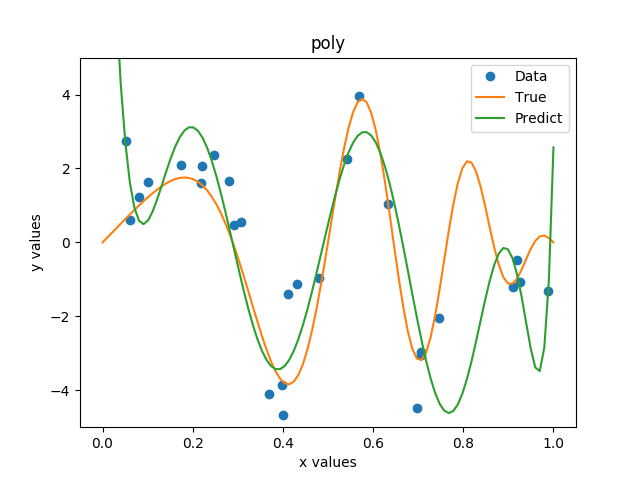
\includegraphics[width=100mm]{../hw3-code/results/a3/a3_bi.png}}
  \subfloat[rbf true vs predict]{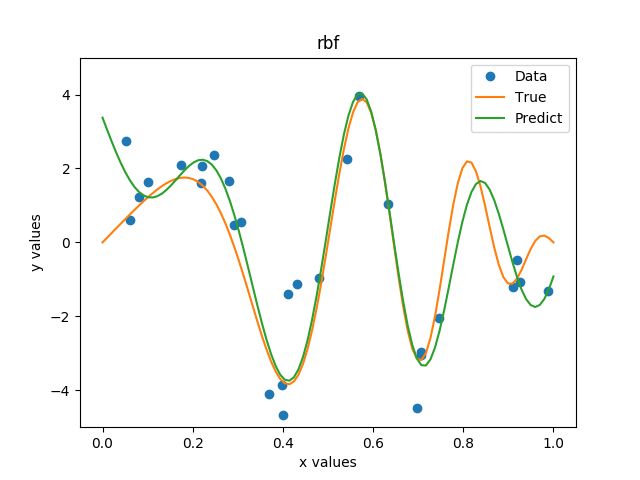
\includegraphics[width=100mm]{../hw3-code/results/a3/a3_bii.png}}
\end{figure}

\newpage

\subsection*{c.}

\begin{figure}[h]
  \centering
  \subfloat[poly with confidence intervals]{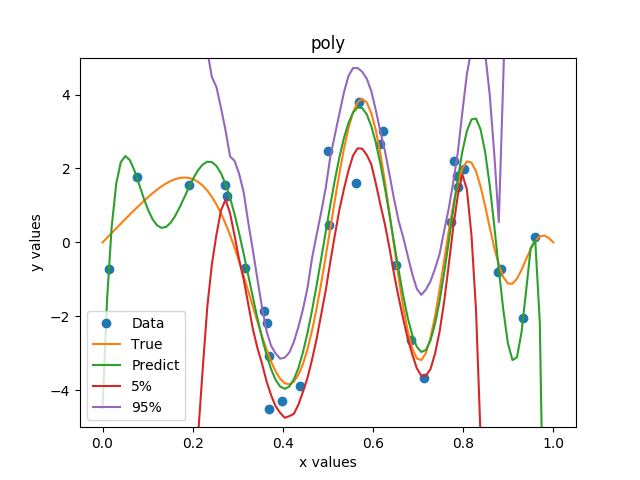
\includegraphics[width=100mm]{../hw3-code/results/a3/a3_ci.png}}
  \subfloat[rbf with confidence intervals]{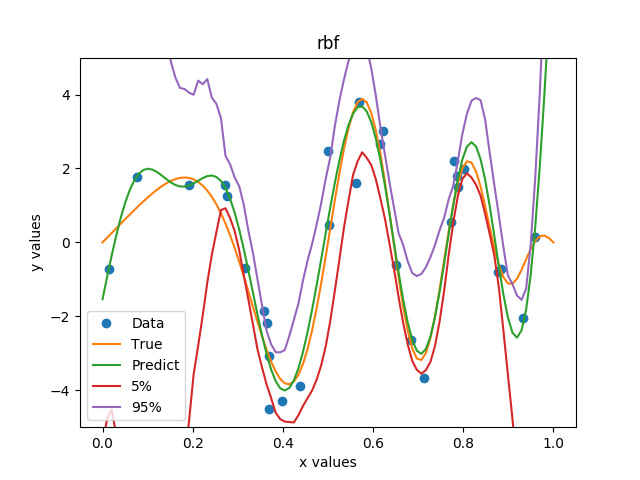
\includegraphics[width=100mm]{../hw3-code/results/a3/a3_cii.png}}
\end{figure}

\subsection*{d.}
\begin{figure}[h]
  \centering
  \subfloat[poly true vs predict]{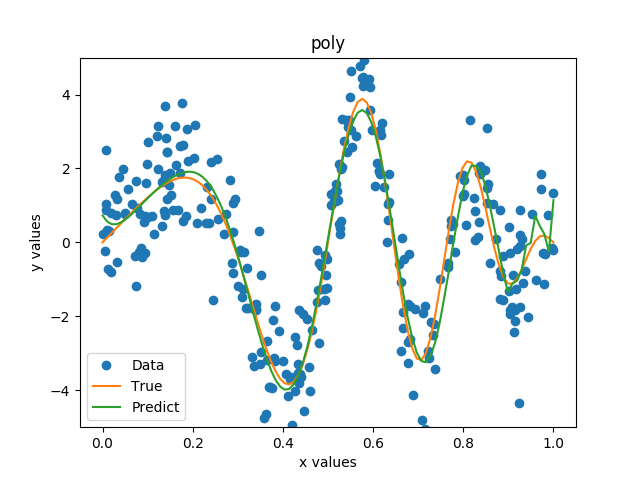
\includegraphics[width=100mm]{../hw3-code/results/a3/a3_d.bi.png}}
  \subfloat[rbf true vs predict]{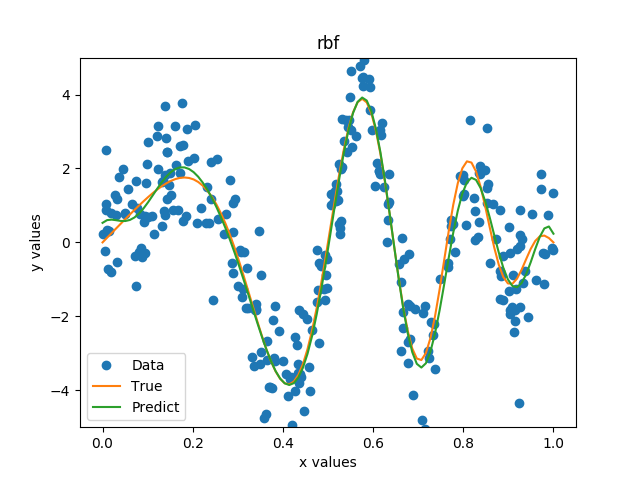
\includegraphics[width=100mm]{../hw3-code/results/a3/a3_d.bii.png}}
\end{figure}
\begin{figure}[h]
  \centering
  \subfloat[poly with confidence intervals]{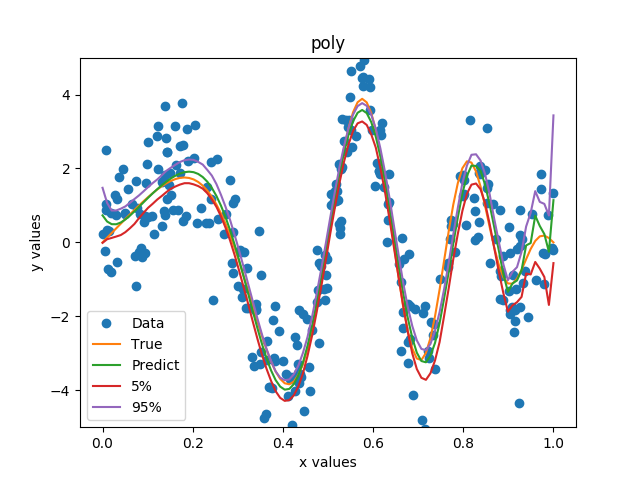
\includegraphics[width=100mm]{../hw3-code/results/a3/a3_d.ci.png}}
  \subfloat[rbf with confidence intervals]{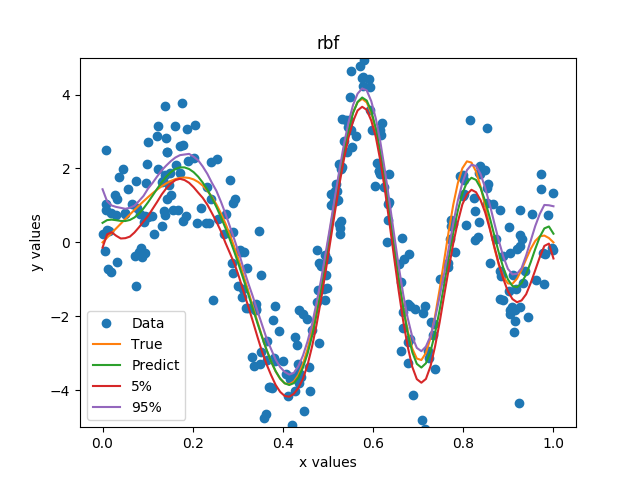
\includegraphics[width=100mm]{../hw3-code/results/a3/a3_d.cii.png}}
\end{figure} 
\newpage
\textbf{poly:} \\
$d: 22.0$ \\
$\lambda: 10^{-7}$ \\ 
\textbf{rbf:} \\
$\gamma: 24.0$ \\
$\lambda: 10^{-4}$

\subsection*{e.}

5\%: 0.33408841623035646 \\
95\%: 0.6405912247916652 \\
Using this confidence interval, which is all positive and does not include 0, there does appear to be statistically significant evidence to suggest that one is the better. Since the way the estimator is constructed has the differences in actual vs predicted values for the polynomial kernel subtracted by that of the rbf kernel, we can see that the differences are greater in the polynomial kernel, which tells us that the rbf kernel seems to be a better predictor in a statistically significant manner.

\begin{verbatim}
# kernel.py
# Applicable code for HW3 A3

import numpy as np

import constants as c
import helpers as h

to_run = {
  "abc" : True,
  "de" : True,
}

def main():

  X, Y, true_f = h.generate_data(30)

  # individual elements over entire matrix
  kf_poly = lambda x, z, d: (1 + x * z) ** d
  kf_rbf = lambda x, z, gamma: np.exp(-gamma * ((x - z) ** 2))

  if to_run["abc"]:
    """
    part (a)
    """

    k_poly = Kernel(X, Y, kf_poly)
    k_rbf = Kernel(X, Y, kf_rbf)

    """
    part (b)
    """

    true_data = [true_f(x_val) for x_val in c.x_list]
    poly_pred_data = k_poly.get_fhat_data(X, Y)
    rbf_pred_data = k_rbf.get_fhat_data(X, Y)

    poly_list = [true_data, poly_pred_data]
    rbf_list = [true_data, rbf_pred_data]

    h.plot_multiple("poly", "a3_bi", X, Y, poly_list, c.pred_labels, c.a3b_ylimits)
    h.plot_multiple("rbf", "a3_bii", X, Y, rbf_list, c.pred_labels, c.a3b_ylimits)

    """
    part (c)
    """

    poly_5, poly_95 = k_poly.bootstrap(c.B)
    rbf_5, rbf_95 = k_rbf.bootstrap(c.B)

    poly_list = [true_data, poly_pred_data, poly_5, poly_95]
    rbf_list = [true_data, rbf_pred_data, rbf_5, rbf_95]

    h.plot_multiple("poly", "a3_ci", X, Y, poly_list, c.pct_labels, c.a3b_ylimits)
    h.plot_multiple("rbf", "a3_cii", X, Y, rbf_list, c.pct_labels, c.a3b_ylimits)

  if to_run["de"]:

    """
    part (d)
    """

    # repeated a
    X, Y, true_f = h.generate_data(300)

    k_poly = Kernel(X, Y, kf_poly, kfold=True)
    k_rbf = Kernel(X, Y, kf_rbf, kfold=True)

    # repeated b
    true_data = [true_f(x_val) for x_val in c.x_list]
    poly_pred_data = k_poly.get_fhat_data(X, Y)
    rbf_pred_data = k_rbf.get_fhat_data(X, Y)

    poly_list = [true_data, poly_pred_data]
    rbf_list = [true_data, rbf_pred_data]

    h.plot_multiple("poly", "a3_d.bi", X, Y, poly_list, c.pred_labels, c.a3b_ylimits)
    h.plot_multiple("rbf", "a3_d.bii", X, Y, rbf_list, c.pred_labels, c.a3b_ylimits)

    # repeated c
    poly_5, poly_95 = k_poly.bootstrap(c.B)
    rbf_5, rbf_95 = k_rbf.bootstrap(c.B)

    poly_list = [true_data, poly_pred_data, poly_5, poly_95]
    rbf_list = [true_data, rbf_pred_data, rbf_5, rbf_95]

    h.plot_multiple("poly", "a3_d.ci", X, Y, poly_list, c.pct_labels, c.a3b_ylimits)
    h.plot_multiple("rbf", "a3_d.cii", X, Y, rbf_list, c.pct_labels, c.a3b_ylimits)

    """
    part (e)
    """

    X, Y, true_f = h.generate_data(c.m)

    poly_pred = k_poly.kernel_rr(X, Y, k_poly.hp, k_poly.lamb)
    rbf_pred = k_rbf.kernel_rr(X, Y, k_rbf.hp, k_rbf.lamb)

    bs_5, bs_95 = get_bootstrap_values(X, Y, poly_pred, rbf_pred)

    print(bs_5)
    print(bs_95)

def get_bootstrap_values(X, Y, poly_pred, rbf_pred, m=c.m, B=c.B):
  
  diff_list = np.zeros(B)

  for i in range(B):
    
    index_samples = np.random.choice(m, m)

    x_b = X[index_samples]
    y_b = Y[index_samples]

    poly_diff = (np.abs(y_b - [poly_pred(x) for x in x_b]) ** 2)
    rbf_diff = (np.abs(y_b - [rbf_pred(x) for x in x_b]) ** 2)

    diff_list[i] = (1 / m) * np.sum(poly_diff - rbf_diff)


  bs_5 = np.percentile(diff_list, 5, axis=0)
  bs_95 = np.percentile(diff_list, 95, axis=0)

  return bs_5, bs_95

class Kernel:
  def __init__(self, X, Y, kernel_func=None, hyperparameter=None, lambda_reg=None, kfold=False):
    self.X = X
    self.Y = Y
    self.kf = kernel_func
    self.hp = hyperparameter
    self.lamb = lambda_reg
    self.kmat = None

    if self.hp is None and self.lamb is None:
      print("setting best hyperparameter, lambda")

      if kfold:
        self.kfold_cv()
      else:
        self.loo_cv()
      

    print("hyperparam: " + str(self.hp))
    print("lambda: " + str(self.lamb))

  def get_fhat_data(self, x, y):
    pred_f = self.kernel_rr(x, y, self.hp, self.lamb)

    return [pred_f(x_val) for x_val in c.x_list]

  def loo_cv(self):
    n = len(self.X)

    error_matrix = np.zeros((len(c.hp_list), len(c.lamb_list)))

    # try every combo and keep track of errors
    for i, hp in enumerate(c.hp_list):
      for j, lamb in enumerate(c.lamb_list):
        for k in range(n):
          X_val = self.X[k]
          Y_val = self.Y[k]
          
          # train without the loo val
          X_train = np.concatenate((self.X[:k], self.X[k + 1:]))
          Y_train = np.concatenate((self.Y[:k], self.Y[k + 1:]))

          f_opt = self.kernel_rr(X_train, Y_train, hp, lamb)

          error_matrix[i][j] += (np.abs(f_opt(X_val) - Y_val) ** 2)
        
        error_matrix[i][j] /= n

    # find minimum index loc
    min_idx = np.argwhere(error_matrix == np.amin(error_matrix))
    min_i = min_idx[0][0]
    min_j = min_idx[0][1]

    assert (error_matrix[min_i][min_j] == np.amin(error_matrix)), "Sanity check min error is accurate"

    self.hp = c.hp_list[min_i]
    self.lamb = c.lamb_list[min_j]
  
  # TODO: refactor this into one module
  def kfold_cv(self):
    n = len(self.X)

    error_matrix = np.zeros((len(c.hp_list), len(c.lamb_list)))

    # try every combo and keep track of errors
    for i, hp in enumerate(c.hp_list):
      for j, lamb in enumerate(c.lamb_list):
        for k in range(c.num_fold):
          fold_start = k * int(n / 10)
          fold_end =  (k + 1) * int(n / 10)

          X_val = self.X[fold_start:fold_end]
          Y_val = self.Y[fold_start:fold_end]

          # train without the loo val
          X_train = np.concatenate((self.X[:fold_start], self.X[fold_end:]))
          Y_train = np.concatenate((self.Y[:fold_start], self.Y[fold_end:]))

          f_opt = self.kernel_rr(X_train, Y_train, hp, lamb)

          error_matrix[i][j] += np.sum(([f_opt(x) for x in X_val] - Y_val) ** 2)

        error_matrix[i][j] /= len(X_val)

    # find minimum index loc
    min_idx = np.argwhere(error_matrix == np.amin(error_matrix))
    min_i = min_idx[0][0]
    min_j = min_idx[0][1]

    assert (error_matrix[min_i][min_j] == np.amin(
        error_matrix)), "Sanity check min error is accurate"

    self.hp = c.hp_list[min_i]
    self.lamb = c.lamb_list[min_j]

  def kernel_rr(self, X_train, Y_train, hp, lamb):
    n = len(X_train)

    kmat = np.fromfunction(lambda i, j: self.kf(X_train[i], X_train[j], hp), shape=(n, n), dtype=int)

    # use optimizer, train
    alpha_opt = np.linalg.solve(kmat + lamb * np.eye(n), Y_train)

    pred_f = lambda x: alpha_opt.dot(self.kf(X_train, x, hp))

    return pred_f

  def bootstrap(self, iterations):
    n = len(self.X)

    B = iterations
    num_x = len(c.x_list)

    fhat_list = np.zeros((B, num_x))

    for i in range(B):
      index_samples = np.random.choice(n, n)

      x_b = self.X[index_samples]
      y_b = self.Y[index_samples]

      fhat_list[i] = np.copy(self.get_fhat_data(x_b, y_b))

    bot_5 = np.percentile(fhat_list, 5, axis=0)
    top_5 = np.percentile(fhat_list, 95, axis=0)

    return bot_5, top_5

if __name__ == "__main__":
  main()

\end{verbatim}

\newpage

}

\section*{A.4}
{\Large 

\subsection*{a.}

Test accuracy = 97.03\% \\
Test loss = 0.0008

\begin{figure}[h]
  \centering
  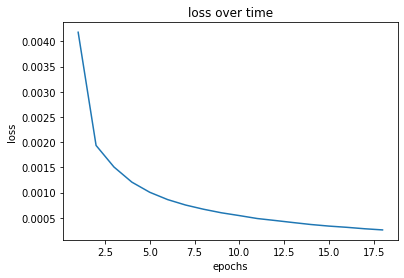
\includegraphics[width=110mm]{../hw3-code/results/a4/a4_a.png}
\end{figure}

\subsection*{b.}

Test accuracy = 96.92\% \\
Test loss = 0.0010

\begin{figure}[h]
  \centering
  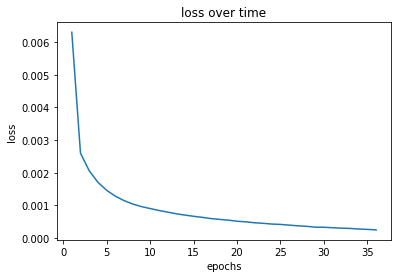
\includegraphics[width=110mm]{../hw3-code/results/a4/a4_b.png}
\end{figure}

\subsection*{c.}

\textbf{Wide and shallow} \\ \\
Number of parameters: $784 \cdot 64 + 64 \cdot 1 + 64 \cdot 10 + 10 \cdot 1 = 50176 + 64 + 640 + 10 = $ \framebox[1.1\width]{\textbf{50890}}  \\
Test accuracy: 97.03\% \\ \\
\textbf{Narrow and deeper} \\ \\
Number of parameters: $784 \cdot 32 + 32 \cdot 1 + 32 \cdot 32 + 32 + 32 \cdot 10 + 10 = 25088 + 32 + 1024 + 32 + 320 + 10 = $ \framebox[1.1\width]{\textbf{26506}} \\
Test accuracy: 96.92\% \\ \\
Although the test accuracies are quite similar in our smaller-scale tests, intuitively, narrow and deeper should be better than wider and shallower. In reality, narrow and deeper networks will be more able to generalize across more data with more layers. Shallower networks work better with less data and on a smaller scale since it can effectively "memorize" on a smaller scale, but not generalize.

\newpage

\begin{verbatim}
# -*- coding: utf-8 -*-
"""cse446_hw3_a4.ipynb

Automatically generated by Colaboratory.

Original file is located at
    https://colab.research.google.com/drive/1_SIbwG3BXMDcx1ZjGFNXcLkcuS4C7G_O
"""

# A4
# Imports

import numpy as np
import matplotlib.pyplot as plt
from mpl_toolkits.mplot3d import Axes3D

import torch
import torch.nn as nn
import torch.nn.functional as F
import torch.optim as optim
import torchvision.datasets as datasets
from torchvision import transforms
from tqdm import tqdm

# Constants

learning_rate = 1E-3

# import MNIST

train_data = datasets.MNIST(root="./data", train=True, download=True, transform=transforms.ToTensor())
test_data = datasets.MNIST(root="./data", train=False, download=True, transform=transforms.ToTensor())

train_loader = torch.utils.data.DataLoader(train_data, batch_size=128, shuffle=True)
test_loader = torch.utils.data.DataLoader(test_data, batch_size=128, shuffle=True)

# Helpers

def initialize_weights(mode, h=64, h_0 = 32, h_1 = 32, m=784, n=10):
  print("Initializing weights for " + mode)
  
  alpha = 1 / np.sqrt(m)
  
  d = m
  k = n
  
  if mode == "a":
    W_0 = nn.init.uniform_(torch.empty(h, d), -alpha, alpha)
    b_0 = nn.init.uniform_(torch.empty(h), -alpha, alpha)
    
    W_1 = nn.init.uniform_(torch.empty(k, h), -alpha, alpha)
    b_1 = nn.init.uniform_(torch.empty(k), -alpha, alpha)
    
    W_0.requires_grad = True
    b_0.requires_grad = True
    W_1.requires_grad = True
    b_1.requires_grad = True
    
    return [W_0, W_1, b_0, b_1]

  if mode == "b":
    W_0 = nn.init.uniform_(torch.empty(h_0, d), -alpha, alpha)    
    b_0 = nn.init.uniform_(torch.empty(h_0), -alpha, alpha)
    
    W_1 = nn.init.uniform_(torch.empty(h_1, h_0), -alpha, alpha)
    b_1 = nn.init.uniform_(torch.empty(h_1), -alpha, alpha)

    W_2 = nn.init.uniform_(torch.empty(k, h_1), -alpha, alpha)
    b_2 = nn.init.uniform_(torch.empty(k), -alpha, alpha)

    W_0.requires_grad = True
    b_0.requires_grad = True
    W_1.requires_grad = True
    b_1.requires_grad = True
    W_2.requires_grad = True
    b_2.requires_grad = True

    return [W_0, W_1, W_2, b_0, b_1, b_2]

def f_1(x, W_0, W_1, b_0, b_1):
  temp = torch.matmul(x, W_0.T) + b_0
  return torch.matmul(F.relu(temp), W_1.T) + b_1

def f_2(x, W_0, W_1, W_2, b_0, b_1, b_2):
  temp1 = F.relu(torch.matmul(x, W_0.T) + b_0)
  temp2 = F.relu(torch.matmul(temp1, W_1.T) + b_1)
  return torch.matmul(temp2, W_2.T) + b_2 

def plot_loss(data, title):
  print("plotting loss")

  epochs = list(range(1, len(data) + 1))

  plt.plot(epochs, data)

  plt.title("loss over time")
  plt.xlabel("epochs")
  plt.ylabel("loss")

  plt.savefig(title)

def train_a(params, learning_rate, h=64, m=784, n=10):
  print("training a")

  W_0, W_1, b_0, b_1 = params[0], params[1], params[2], params[3]  

  optimizer = optim.Adam(params, lr=learning_rate)
  
  loss_data = []
  
  while True:

    acc = 0.
    loss_sum = 0.

    for x, y in tqdm(train_loader):
      x = x.view(-1, m)

      predictions = f_1(x, W_0, W_1, b_0, b_1)

      acc += torch.sum(torch.argmax(predictions, dim=1) == y)

      loss = F.cross_entropy(predictions, y)
      optimizer.zero_grad()
      loss.backward()
      optimizer.step()

      loss_sum += loss
    
    loss_data.append(loss_sum / len(train_loader.dataset))
    acc = acc / len(train_loader.dataset)

    if acc >= 0.99:
      break
  
  return loss_data, [W_0, W_1, b_0, b_1]

def test_a(params):
  print("testing a")

  acc = 0.
  loss_sum = 0.

  W_0, W_1, b_0, b_1 = params[0], params[1], params[2], params[3]

  for x, y in tqdm(test_loader):
    x = torch.flatten(x, start_dim=1, end_dim=3)

    predictions = f_1(x, W_0, W_1, b_0, b_1)

    acc += torch.sum(torch.argmax(predictions, dim=1) == y)
    loss_sum += F.cross_entropy(predictions, y)
  
  acc /= len(test_loader.dataset)
  loss_sum /= len(test_loader.dataset)

  return acc, loss_sum

######################## part (a) ########################

params = initialize_weights("a")
a_train_loss, params = train_a(params, learning_rate)
plot_loss(a_train_loss, "a4_a")

a_test_acc, a_test_loss = test_a(params)
print(a_test_acc)
print(a_test_loss)

def train_b(params, learning_rate, h=32, m=784):
  print("training b")

  W_0, W_1, W_2, b_0, b_1, b_2 = params[0], params[1], params[2], params[3], params[4], params[5]

  optimizer = optim.Adam(params, lr=learning_rate)
    
  acc_data = []
  loss_data = []

  while True:

    acc = 0.
    loss_sum = 0.

    for x, y in tqdm(train_loader):
      x = x.view(-1, m)

      predictions = f_2(x, W_0, W_1, W_2, b_0, b_1, b_2)

      acc += torch.sum(torch.argmax(predictions, dim=1) == y)

      loss = F.cross_entropy(predictions, y)
      optimizer.zero_grad()
      loss.backward()
      optimizer.step()

      loss_sum += loss
    
    loss_data.append(loss_sum / len(train_loader.dataset))
    acc = acc / len(train_loader.dataset)
    
    if acc >= 0.99:
      break
  
  return loss_data, [W_0, W_1, W_2, b_0, b_1, b_2]

def test_b(params):
  print("testing b")

  acc = 0.
  loss_sum = 0.
  
  W_0, W_1, W_2, b_0, b_1, b_2 = params[0], params[1], params[2], params[3], params[4], params[5]
  
  for x, y in tqdm(test_loader):
    x = torch.flatten(x, start_dim=1, end_dim=3)

    predictions = f_2(x, W_0, W_1, W_2, b_0, b_1, b_2)

    acc += torch.sum(torch.argmax(predictions, dim=1) == y)
    loss_sum += F.cross_entropy(predictions, y)
  
  acc /= len(test_loader.dataset)
  loss_sum /= len(test_loader.dataset)

  return acc, loss_sum

######################## part (b) ########################
params = initialize_weights("b")
b_train_loss, params = train_b(params, learning_rate)
plot_loss(b_train_loss, "a4_b")

b_test_acc, b_test_loss = test_b(params)
print(b_test_acc)
print(b_test_loss)

\end{verbatim}

}



\newpage
\section*{A.5}
{\Large 

For (a) and (b), the hyperparameters used were as follows: \\
Learning rate = $10^{-3}$ \\
Batch size = 128 \\
Epochs = 20

\subsection*{a.}

Highest validation accuracy = 79.60\% \\
Test accuracy = 80.62\% \\
Test loss = 0.5628582025527954

\begin{figure}[h]
  \centering
  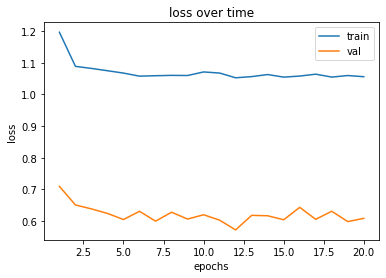
\includegraphics[width=150mm]{../hw3-code/results/a5/a5_a.png}
\end{figure}

\newpage

\subsection*{b.}

\begin{figure}[h]
  \centering
  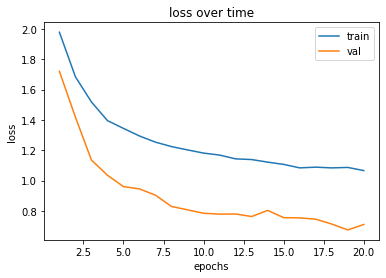
\includegraphics[width=150mm]{../hw3-code/results/a5/a5_b.png}
\end{figure}

Highest validation accuracy = 77.42\% \\
Test accuracy = 76.34\% \\
Test loss = 0.7033713958740234

\newpage

\begin{verbatim}
# -*- coding: utf-8 -*-
"""cse446_hw3_a5.ipynb

Automatically generated by Colaboratory.

Original file is located at
    https://colab.research.google.com/drive/11aNA4mlWdyL4rPJEsDzZmBsNRF1as1nm
"""

# A5
# Imports

import copy
import os
import numpy as np
import matplotlib.pyplot as plt
from mpl_toolkits.mplot3d import Axes3D

import torch
import torch.nn as nn
import torch.nn.functional as F
import torch.optim as optim
import torchvision.datasets as datasets
import torchvision.models as models
import torch.utils.data as data
from torchvision import transforms
from tqdm import tqdm

# Constants
device = "cuda" if torch.cuda.is_available() else "cpu"

learning_rate = 1E-3
epochs = 20
val_pct = 0.1
batch_size = 128

labels = ['train', 'val']

data_transforms = {
      'train': transforms.Compose([
          transforms.RandomResizedCrop(224),
          transforms.RandomHorizontalFlip(),
          transforms.ToTensor(),
          transforms.Normalize([0.485, 0.456, 0.406], [0.229, 0.224, 0.225])
      ]),
      'val': transforms.Compose([
          transforms.Resize(256),
          transforms.CenterCrop(224),
          transforms.ToTensor(),
          transforms.Normalize([0.485, 0.456, 0.406], [0.229, 0.224, 0.225])
      ]),
      # yeah this is the same for now
      'test': transforms.Compose([
          transforms.Resize(256),
          transforms.CenterCrop(224),                                
          transforms.ToTensor(),
          transforms.Normalize([0.485, 0.456, 0.406], [0.229, 0.224, 0.225])
      ]),
  }

# Helpers

def get_dataset():

  train_data = datasets.CIFAR10(root="./data/train", train=True, download=True, transform=data_transforms['train'])
  val_data = datasets.CIFAR10(root="./data/val", train=True, download=True, transform=data_transforms['val'])
  test_data = datasets.CIFAR10(root="./data/test", train=False, download=True, transform=data_transforms['test'])

  # break up into training/validation
  train_idx = np.random.permutation(np.arange(len(train_data)))
  val_data = data.Subset(val_data, train_idx[0:int(val_pct * len(train_data))])
  train_data = data.Subset(train_data, train_idx[int(val_pct * len(train_data)):])

  # dataloaders
  train_loader = data.DataLoader(train_data, batch_size=batch_size, shuffle=True)
  val_loader = data.DataLoader(val_data, batch_size=batch_size, shuffle=True)
  test_loader = data.DataLoader(test_data, batch_size=batch_size, shuffle=True)

  return train_loader, val_loader, test_loader

train_loader, val_loader, test_loader = get_dataset()

def plot_train_val_loss(train_data, val_data, title):
  print("plotting loss")

  epochs = list(range(1, len(train_data) + 1))

  print(train_data)
  print(val_data)

  plt.plot(epochs, train_data)
  plt.plot(epochs, val_data)

  plt.title("loss over time")
  plt.xlabel("epochs")
  plt.ylabel("loss")
  
  plt.legend(labels)

  plt.savefig(title)

def train_model(model, criterion, optimizer, num_epochs=20):
  train_loss_list = []
  val_loss_list = []
  val_acc_list = []

  best_model_wts = copy.deepcopy(model.state_dict())
  best_acc = 0.0

  for epoch in range(num_epochs):

    train_loss = 0.0
    model.train()

    for inputs, labels in tqdm(train_loader):
      inputs, labels = inputs.to(device), labels.to(device)
      optimizer.zero_grad()
      
      with torch.set_grad_enabled(True):
        outputs = model(inputs)
        _, preds = torch.max(outputs, 1)
        loss = criterion(outputs, labels)
        loss.backward()
        optimizer.step()

      train_loss += float(loss.item())
    
    train_loss /= len(train_loader.dataset)
    print(train_loss)
    train_loss_list.append(train_loss)

    val_loss = 0.0
    val_acc = 0.0
    model.eval()
        
    for inputs, labels in tqdm(val_loader):
      inputs, labels = inputs.to(device), labels.to(device)
      optimizer.zero_grad()

      with torch.set_grad_enabled(False):
        outputs = model(inputs)
        _, preds = torch.max(outputs, 1)
        loss = criterion(outputs, labels)

      val_loss += float(loss.item())
      val_acc += torch.sum(preds == labels.data)
        
    val_loss /= len(val_loader.dataset)
    val_acc = val_acc.double() / len(val_loader.dataset)
    
    val_loss_list.append(val_loss)
    val_acc_list.append(val_acc)

    if val_acc > best_acc:
      best_acc = val_acc
      best_model_wts = copy.deepcopy(model.state_dict())
  
  model.load_state_dict(best_model_wts)
  return model, train_loss_list, val_loss_list, val_acc_list

def test_alex(model):
  acc = 0.
  loss_sum = 0.
  total = 0.

  model.eval()

  with torch.no_grad():
    for inputs, labels in tqdm(test_loader):
      inputs, labels = inputs.to(device), labels.to(device)

      outputs = model(inputs)
      _, preds = torch.max(outputs.data, 1)
      loss = criterion(outputs, labels)

      loss_sum += float(loss.item())
      acc += (preds == labels).sum().item()
      total += labels.size(0)
        
  loss_sum /= total
  acc /= total

  return acc, loss_sum

######################## part (a) ########################

fixed_model = models.alexnet(pretrained=True)
for param in fixed_model.parameters():
  param.requires_grad = False
fixed_model.classifier[6] = nn.Linear(4096, 10)
fixed_model = fixed_model.to(device)

criterion = nn.CrossEntropyLoss(reduction='sum')
optimizer = torch.optim.Adam(fixed_model.parameters(), learning_rate)

fixed_model, a_train_loss, a_val_loss, a_val_acc = train_model(fixed_model, criterion, optimizer, epochs)
a_test_acc, a_test_loss = test_alex(fixed_model)

plot_train_val_loss(a_train_loss, a_val_loss, "a5_a.png")
print(max(a_val_acc))
print(a_test_acc)
print(a_test_loss)

######################## part (b) ########################

fine_model = models.alexnet(pretrained=True)
fine_model.classifier[6] = nn.Linear(4096, 10)
fine_model = fine_model.to(device)

criterion = nn.CrossEntropyLoss(reduction='sum')
optimizer = torch.optim.Adam(fine_model.parameters(), learning_rate)

fine_model, b_train_loss, b_val_loss, b_val_acc = train_model(fine_model, criterion, optimizer, epochs)
b_test_acc, b_test_loss = test_alex(fine_model)

plot_train_val_loss(b_train_loss, b_val_loss, "a5_b.png")
print(max(b_val_acc))
print(b_test_acc)
print(b_test_loss)
\end{verbatim}

\newpage

}

\section*{A.6}
{\Large 

\framebox[1.1\width]{\textbf{Applicable output can be found in a6a.txt / a6b.txt / a6c.txt / a6d.txt,}} \\
\framebox[1.1\width]{\textbf{which I did not paste in due to its length}}

\subsection*{a.}

\textbf{Hyperparameters tested:} \\
Learning rate = [10E-2, 10E-3, 10E-4] \\
Batch size = [5, 25, 100, 500] \\

\begin{figure}[h]
  \centering
  \subfloat[training]{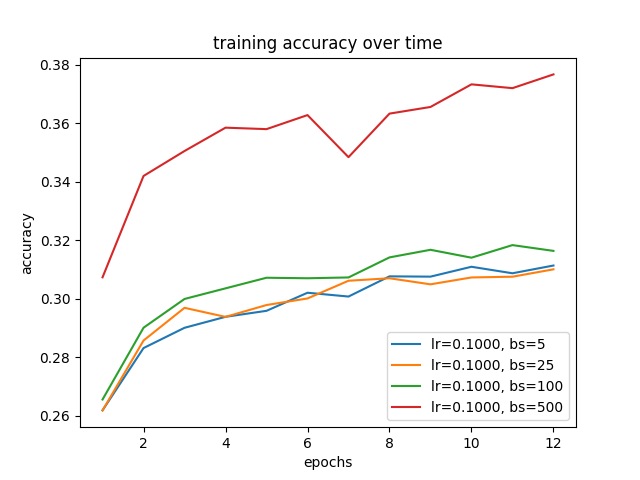
\includegraphics[width=90mm]{../hw3-code/results/a6a/a6_a_t0.png}}
  \subfloat[validation]{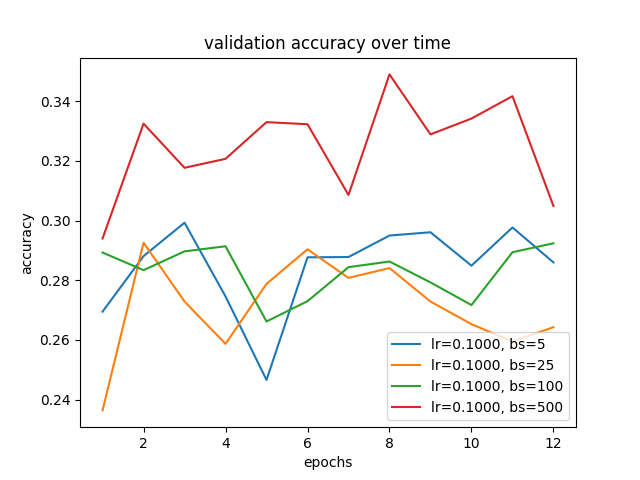
\includegraphics[width=90mm]{../hw3-code/results/a6a/a6_a_v0.png}}
\end{figure}

\begin{figure}[h]
  \centering
  \subfloat[training]{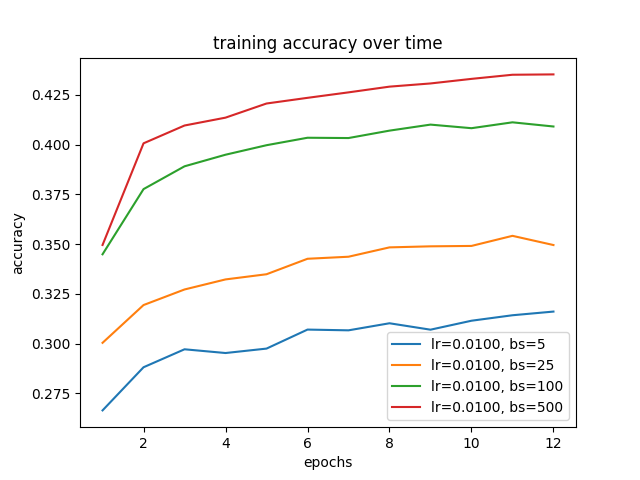
\includegraphics[width=90mm]{../hw3-code/results/a6a/a6_a_t1.png}}
  \subfloat[validation]{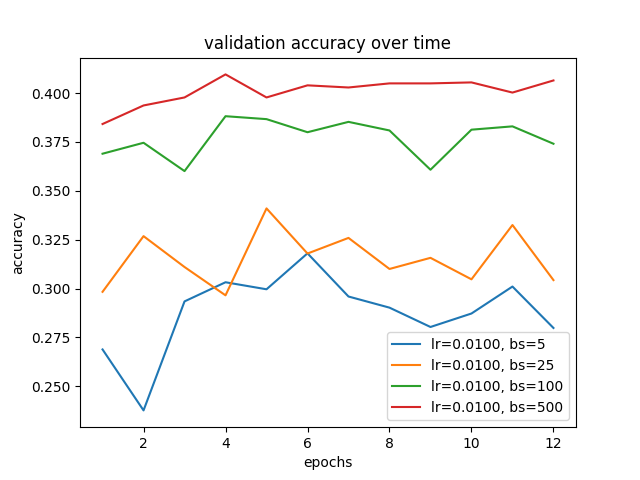
\includegraphics[width=90mm]{../hw3-code/results/a6a/a6_a_v1.png}}
\end{figure}

\begin{figure}[t]
  \centering
  \subfloat[training]{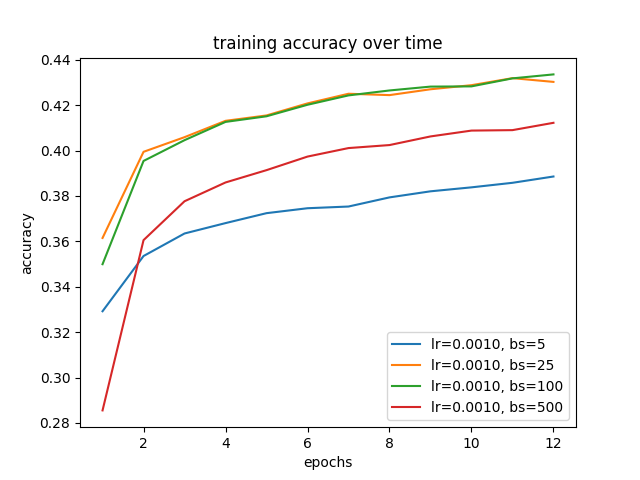
\includegraphics[width=90mm]{../hw3-code/results/a6a/a6_a_t2.png}}
  \subfloat[validation]{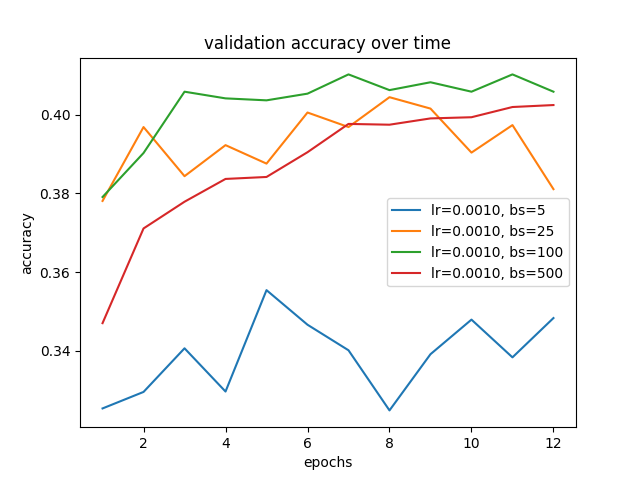
\includegraphics[width=90mm]{../hw3-code/results/a6a/a6_a_v2.png}}
\end{figure}
\newpage

\textbf{Best hyperparameters:} \\
Learning rate = 0.001 \\
Batch size = 100 \\
Train accuracy: 43.3525\% \\
Test accuracy: 40.93\%

\begin{figure}[h]
  \centering
  \subfloat[best hyperparameters training]{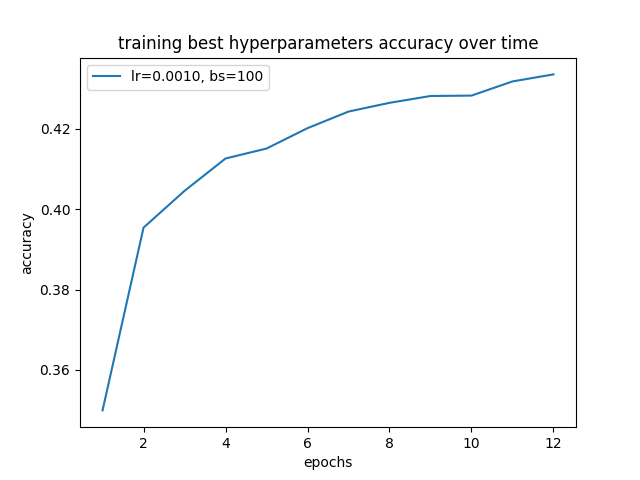
\includegraphics[width=100mm]{../hw3-code/results/a6a/a6_a_tb.png}}
  \subfloat[best hyperparameters validation]{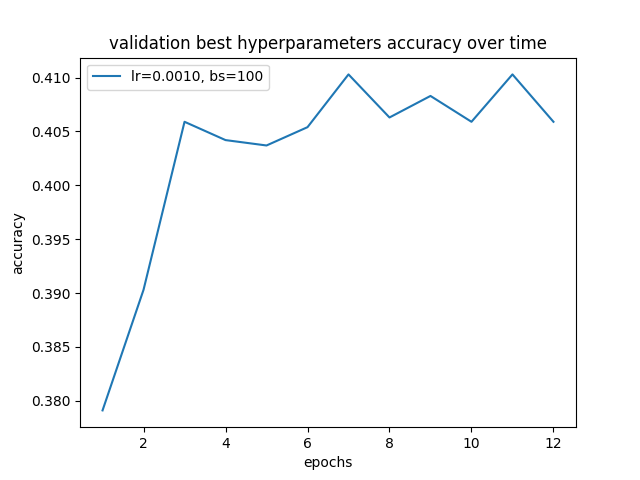
\includegraphics[width=100mm]{../hw3-code/results/a6a/a6_a_vb.png}}
\end{figure}

\subsection*{b.}

\textbf{Hyperparameters tested:} \\
Learning rate = [10E-3, 10E-4] \\
Momentum = [0.8, 0.85, 0.9] \\
M = [100, 200, 300] \\ \\
Keeping constant, as we learned previously: \\
Batch size = 100

\begin{figure}[h]
  \centering
  \subfloat[training]{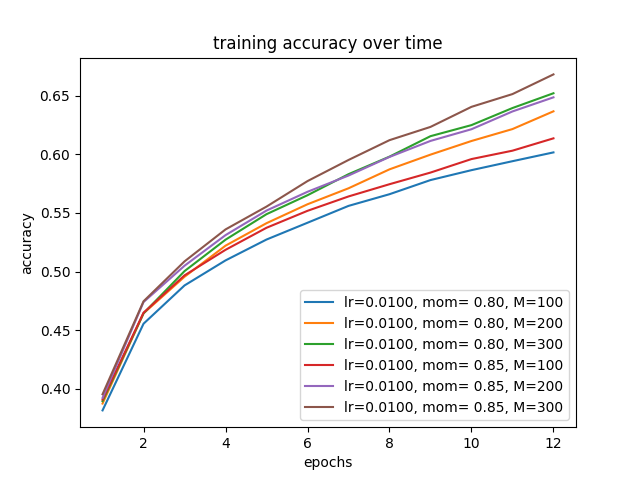
\includegraphics[width=90mm]{../hw3-code/results/a6b/a6_b_t0.png}}
  \subfloat[validation]{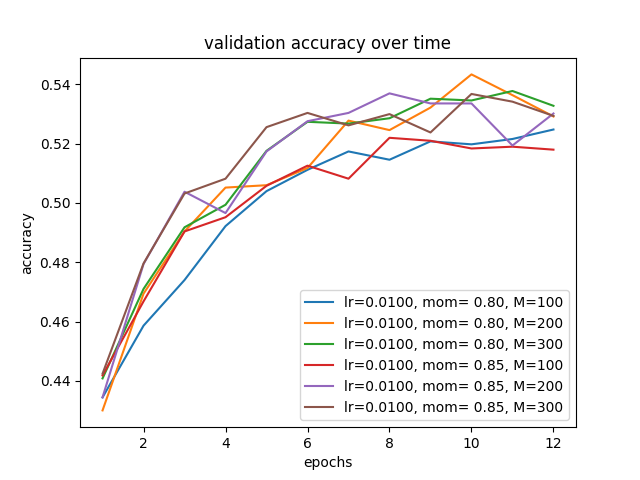
\includegraphics[width=90mm]{../hw3-code/results/a6b/a6_b_v0.png}}
\end{figure}

\begin{figure}[h]
  \centering
  \subfloat[training]{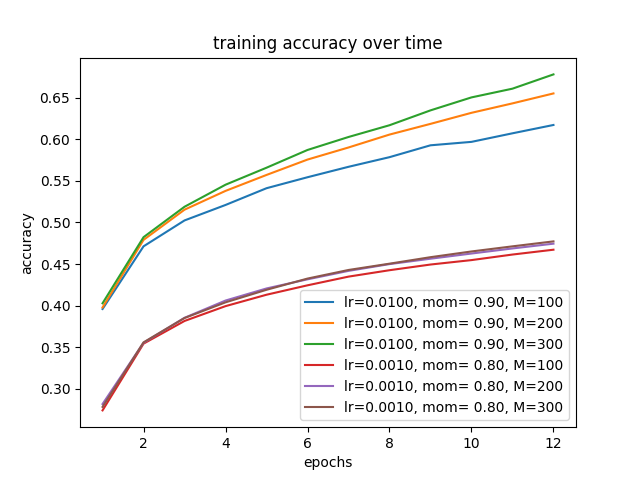
\includegraphics[width=90mm]{../hw3-code/results/a6b/a6_b_t1.png}}
  \subfloat[validation]{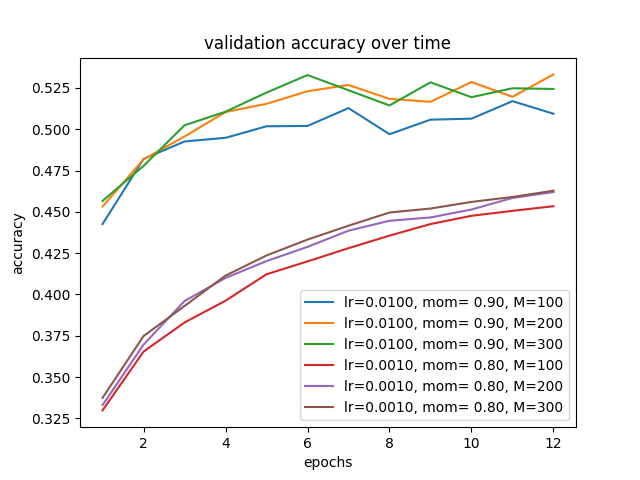
\includegraphics[width=90mm]{../hw3-code/results/a6b/a6_b_v1.png}}
\end{figure}

\begin{figure}[h]
  \centering
  \subfloat[training]{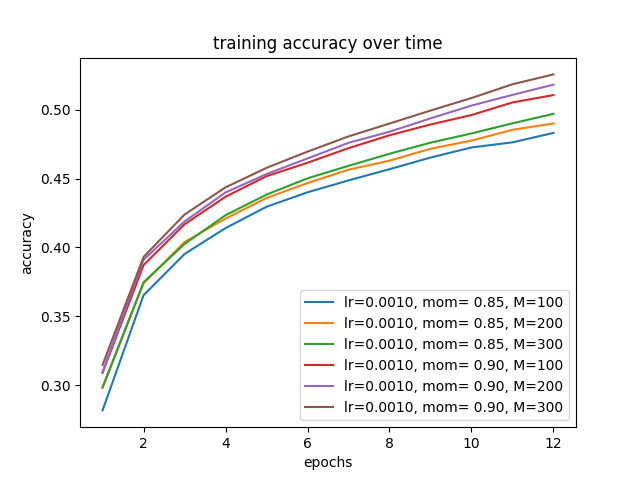
\includegraphics[width=100mm]{../hw3-code/results/a6b/a6_b_t2.png}}
  \subfloat[validation]{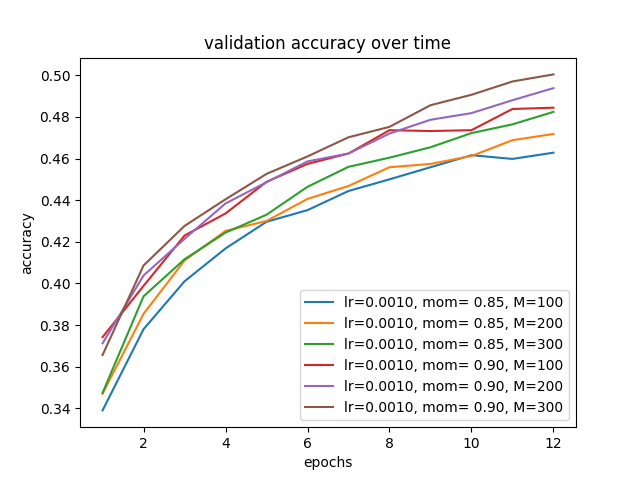
\includegraphics[width=100mm]{../hw3-code/results/a6b/a6_b_v2.png}}
\end{figure}

\newpage 

\textbf{Best hyperparameters:} \\
Learning rate = 0.01 \\
Momentum = 0.90 \\
M = 300 \\
Train accuracy: $\sim$ 70.01\%\\
Test accuracy: 51.72\%

\begin{figure}[h]
  \centering
  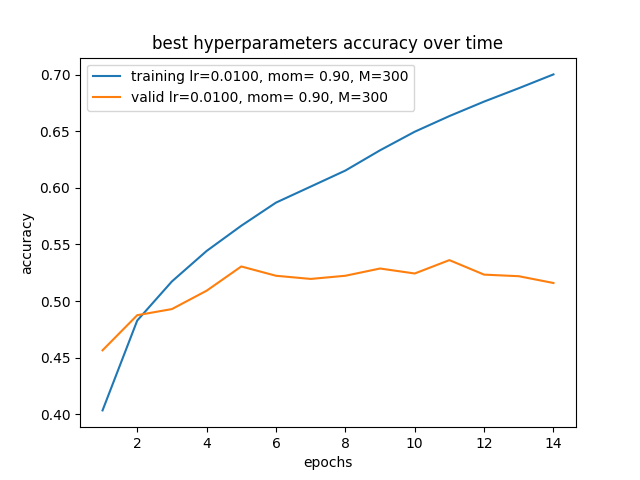
\includegraphics[width=130mm]{../hw3-code/results/a6b/a6_b_best.png}
\end{figure}

\subsection*{c.}

\textbf{Hyperparameters tested:} \\
Learning rate = [10E-3, 10E-4] \\
Momentum = [0.8, 0.85, 0.9] \\ \\ 
Keeping constant, as we learned previously: \\
Batch size = 100 \\
M = 100, k = 5, N = 14 as suggested \\

\begin{figure}[h]
  \centering
  \subfloat[training]{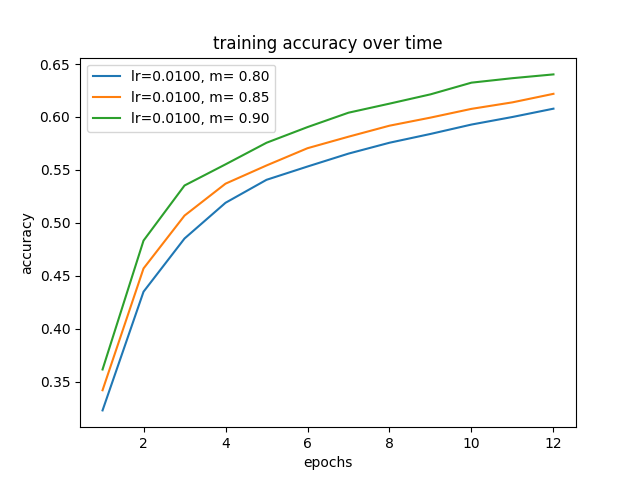
\includegraphics[width=90mm]{../hw3-code/results/a6c/a6_c_t0.png}}
  \subfloat[validation]{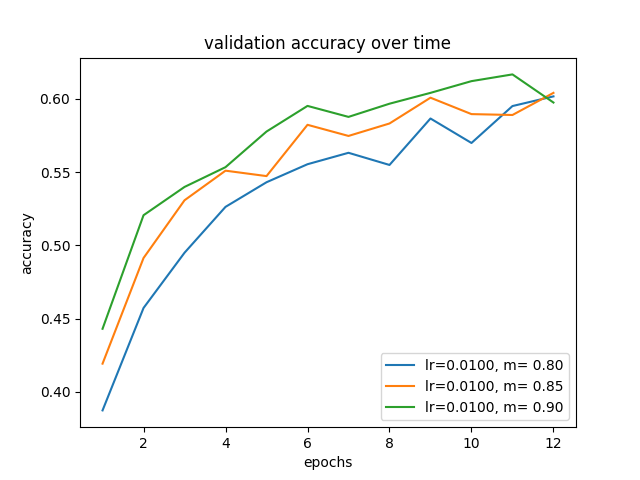
\includegraphics[width=90mm]{../hw3-code/results/a6c/a6_c_v0.png}}
\end{figure}

\begin{figure}[h]
  \centering
  \subfloat[training]{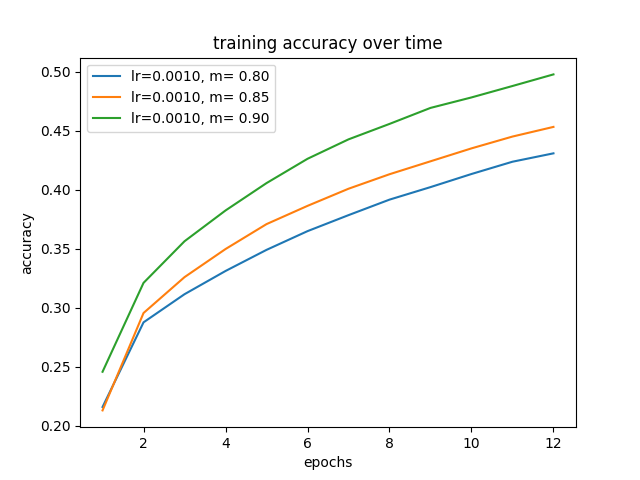
\includegraphics[width=90mm]{../hw3-code/results/a6c/a6_c_t1.png}}
  \subfloat[validation]{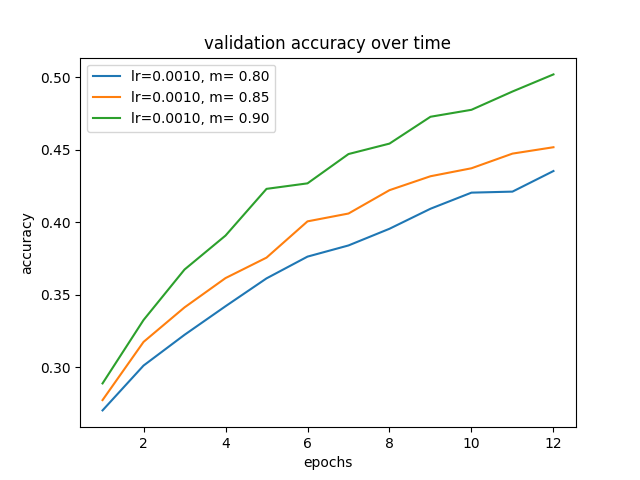
\includegraphics[width=90mm]{../hw3-code/results/a6c/a6_c_v1.png}}
\end{figure}

\newpage

\textbf{Best hyperparameters:} \\ 
Learning rate = 0.01 \\ 
Momentum = 0.90 \\
Train accuracy: 70.0775\% \\
Test accuracy: 63.42\%

\begin{figure}[h]
  \centering
  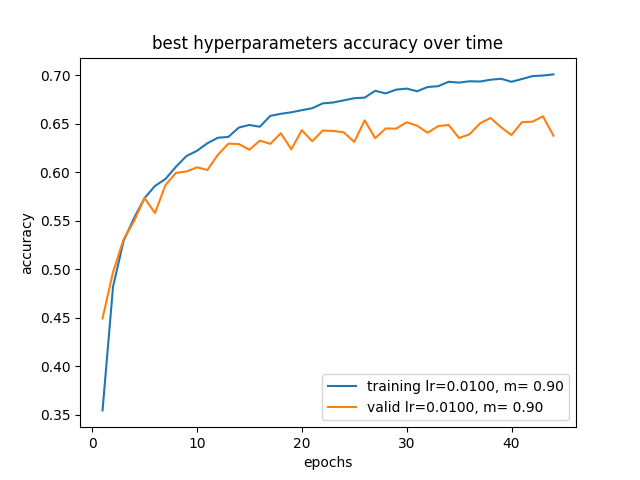
\includegraphics[width=130mm]{../hw3-code/results/a6c/a6_c_best.png}
\end{figure}

\newpage

\subsection*{d.}

\textbf{Hyperparameters tested:} \\
Momentum = [0.8, 0.9] \\
Linear layer 1 output size = [120, 160] \\ 
Linear layer 2 output size = [84, 100] \\
2D Convolution layer 1 output channel size = [16, 32] \\ \\
Keeping constant, as we learned previously: \\
Learning rate = 10E-3 \\
Batch size = 100 \\
All other parameters the same as in the tutorial 

\begin{figure}[h]
  \centering
  \subfloat[training]{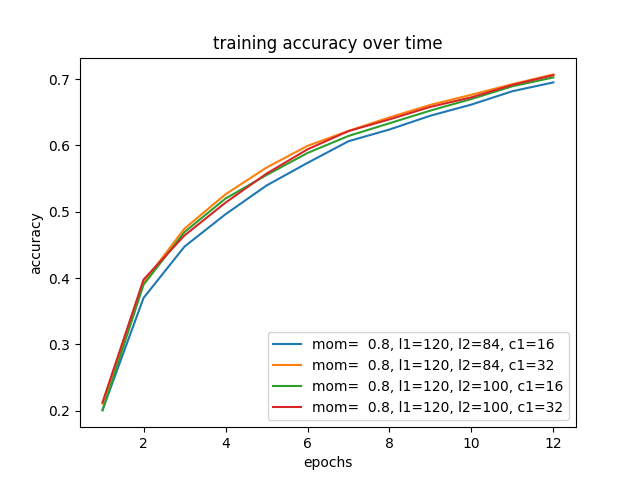
\includegraphics[width=80mm]{../hw3-code/results/a6d/a6_d_t0.png}}
  \subfloat[validation]{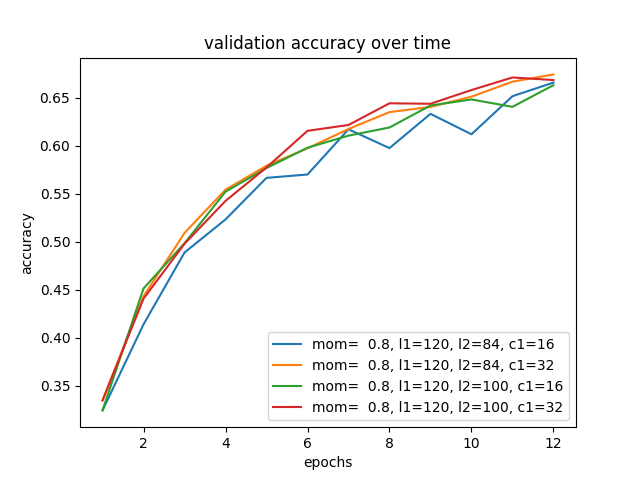
\includegraphics[width=80mm]{../hw3-code/results/a6d/a6_d_v0.png}}
\end{figure}

\begin{figure}[h]
  \centering
  \subfloat[training]{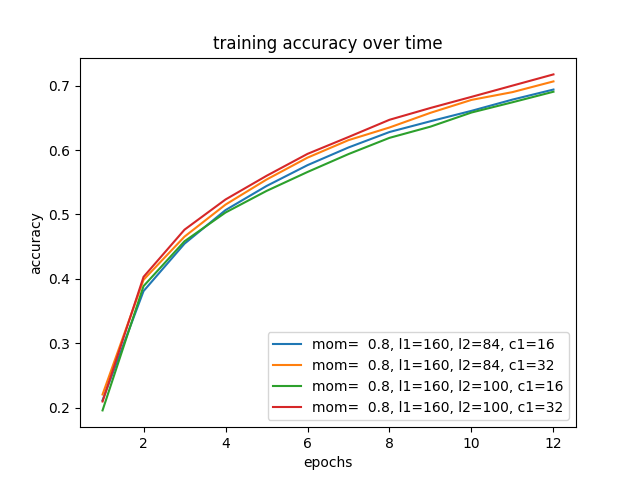
\includegraphics[width=80mm]{../hw3-code/results/a6d/a6_d_t1.png}}
  \subfloat[validation]{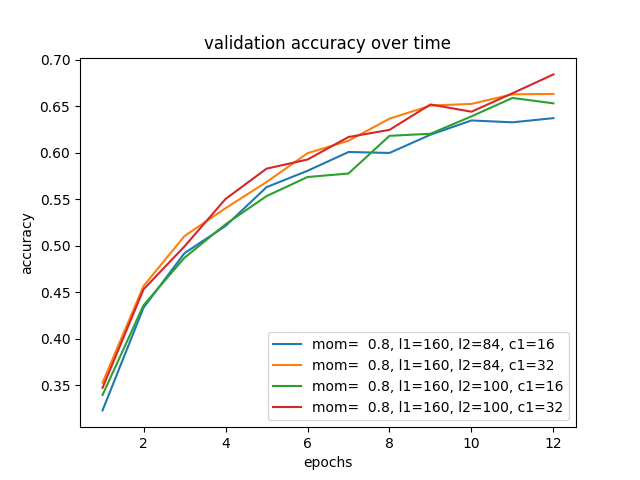
\includegraphics[width=80mm]{../hw3-code/results/a6d/a6_d_v1.png}}
\end{figure}

\begin{figure}[h]
  \centering
  \subfloat[training]{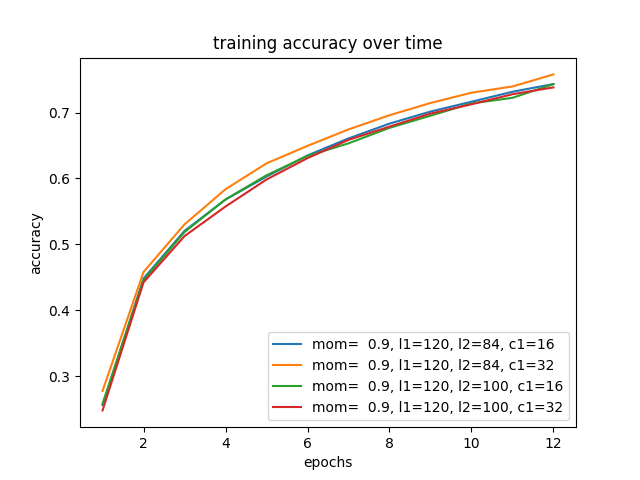
\includegraphics[width=90mm]{../hw3-code/results/a6d/a6_d_t2.png}}
  \subfloat[validation]{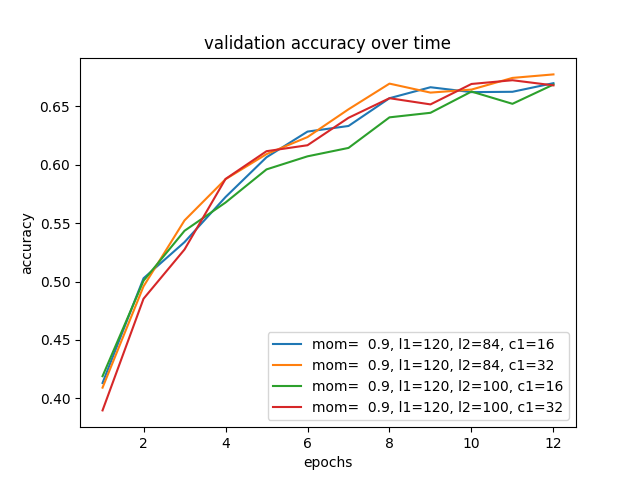
\includegraphics[width=90mm]{../hw3-code/results/a6d/a6_d_v2.png}}
\end{figure}

\begin{figure}[h]
  \centering
  \subfloat[training]{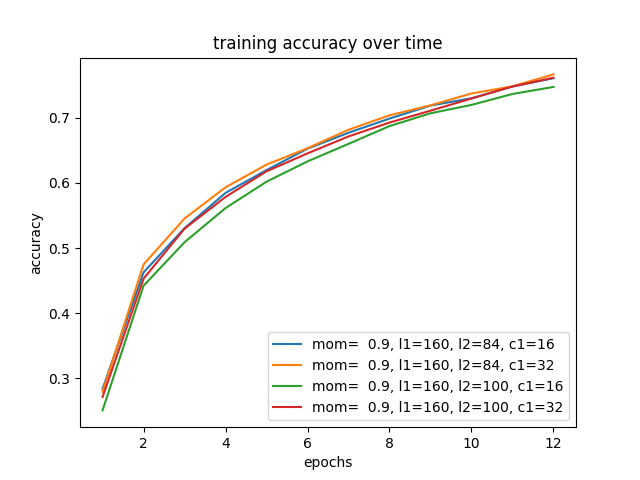
\includegraphics[width=90mm]{../hw3-code/results/a6d/a6_d_t3.png}}
  \subfloat[validation]{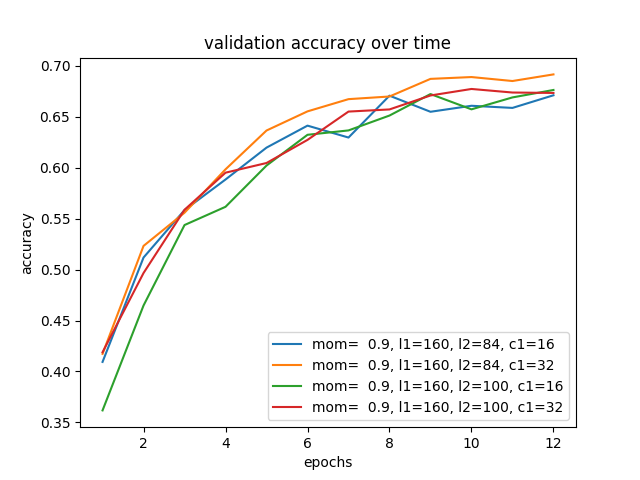
\includegraphics[width=90mm]{../hw3-code/results/a6d/a6_d_v3.png}}
\end{figure}

\newpage

\textbf{Best hyperparameters:} \\
Momentum = 0.80 \\
L1 size = 160 \\
L2 size = 100 \\
C1 size = 32 \\
Train accuracy: 80.1\% \\
Test accuracy: 70.41\%

\begin{figure}[h]
  \centering
  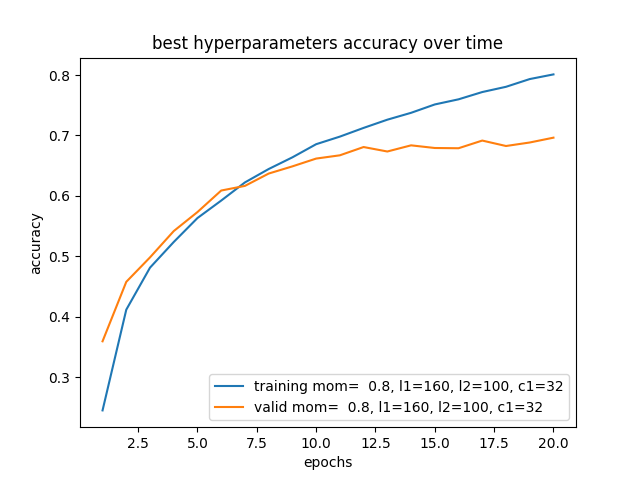
\includegraphics[width=130mm]{../hw3-code/results/a6d/a6_d_best.png}
\end{figure}

\newpage

\begin{verbatim}
# -*- coding: utf-8 -*-
"""cse446_hw3_a6.ipynb

Automatically generated by Colaboratory.

Original file is located at
    https://colab.research.google.com/drive/1wMQV1BlCHBrWj8jnSL_if1u43x7lfAIO
"""

# Commented out IPython magic to ensure Python compatibility.
# %matplotlib inline

import os
import numpy as np
import matplotlib.pyplot as plt
from mpl_toolkits.mplot3d import Axes3D

import torch
import torch.nn as nn
import torch.nn.functional as F
import torch.optim as optim
import torchvision as torchvision
import torchvision.datasets as datasets
import torchvision.models as models
import torch.utils.data as data
from torchvision import transforms
from tqdm import tqdm

# Constants 

device = "cuda" if torch.cuda.is_available() else "cpu"

valid_pct = 0.2
M_B = 100
M_C = 100
k = 5
N = 14

# Helpers and loading data

def get_dataset():

  transform = transforms.Compose(
      [transforms.ToTensor(),
      transforms.Normalize((0.5, 0.5, 0.5), (0.5, 0.5, 0.5))])

  trainset = datasets.CIFAR10(root='./data', train=True,
                                          download=True, transform=transform)
  trainset, validset = data.random_split(trainset, [int((1.0 - valid_pct) * len(trainset)),
                                                    int(valid_pct * len(trainset))])
  testset = datasets.CIFAR10(root='./data', train=False,
                                        download=True, transform=transform)

  return trainset, validset, testset

trainset, validset, testset = get_dataset()

def plot_acc(dataset, legends, filename, set_type, epochs=12):

  epoch_list = list(range(1, epochs + 1))

  print(dataset)

  for item in dataset:
    plt.plot(epoch_list, item)

  plt.title(set_type + " accuracy over time")
  plt.xlabel("epochs")
  plt.ylabel("accuracy")
  
  plt.legend(legends)

  plt.savefig(filename)

# Network definitions

# A_Net
class A_Net(nn.Module):
  def __init__(self):
    super().__init__()
    # Note that 3072 = 32 * 32 * 3, so need to flatten
    self.W = nn.Linear(3072, 10)

  def forward(self, x):
    x = x.view(-1, 32 * 32 * 3)
    return self.W(x)

# B_Net
class B_Net(nn.Module):
  def __init__(self, M_B=M_B):
    super().__init__()
    self.W1 = nn.Linear(3072, M_B)
    self.W2 = nn.Linear(M_B, 10)

  def forward(self, x):
    x = x.view(-1, 32 * 32 * 3)
    x = self.W1(x)
    x = F.relu(x)
    return self.W2(x)

# C_Net
class C_Net(nn.Module):
  def __init__(self, M=M_C, k=k, N=N):
    super().__init__()
    # 3 image input channels, M filters, kxk convolution
    self.conv = nn.Conv2d(3, M, k)
    self.pool = nn.MaxPool2d(N, N)
    # fc layer
    self.W2 = nn.Linear(int(M * ((int(33 - k) / int(N)) ** 2)), 10)

  def forward(self, x):
    x = F.relu(self.conv(x))
    x = self.pool(x)
    x = torch.flatten(x, start_dim=1, end_dim=3)
    return self.W2(x)

class D_Net(nn.Module):
    def __init__(self, c1, l1, l2):
        super().__init__()
        self.conv1 = nn.Conv2d(3, c1, 5)
        self.pool = nn.MaxPool2d(2, 2)
        self.conv2 = nn.Conv2d(c1, 16, 5)
        self.fc1 = nn.Linear(16 * 5 * 5, l1)
        self.fc2 = nn.Linear(l1, l2)
        self.fc3 = nn.Linear(l2, 10)

    def forward(self, x):
        x = self.pool(F.relu(self.conv1(x)))
        x = self.pool(F.relu(self.conv2(x)))
        x = torch.flatten(x, 1) # flatten all dimensions except batch
        x = F.relu(self.fc1(x))
        x = F.relu(self.fc2(x))
        x = self.fc3(x)
        return x

def train(model, learning_rate, batch_size=100, momentum=0.9, epochs=12):

  trainloader = data.DataLoader(trainset, batch_size=batch_size,
                                shuffle=True, num_workers=2)
  validloader = data.DataLoader(validset, batch_size=batch_size,
                                shuffle=True, num_workers=2)

  criterion = nn.CrossEntropyLoss()
  optimizer = optim.SGD(model.parameters(), lr=learning_rate, momentum=momentum)

  local_train_list = []
  local_valid_list = []

  for epoch in range(epochs):  # loop over the dataset multiple times

    train_correct = 0.0
    valid_correct = 0.0
    train_total = 0.0
    valid_total = 0.0

    torch.set_grad_enabled(True)
    model.train()

    # for inputs, labels in tqdm(trainloader):
    for inputs, labels in trainloader:

      inputs = inputs.to(device)
      labels = labels.to(device)

      # zero the parameter gradients
      optimizer.zero_grad()

      # forward + backward + optimize
      outputs = model.forward(inputs)
      loss = criterion(outputs, labels)
      loss.backward()
      optimizer.step()
        
      train_total += labels.size(0)
      train_correct += (torch.argmax(outputs, dim=1) == labels).sum().item()
    
    torch.no_grad()
    model.eval()

    # for inputs, labels in tqdm(validloader):
    for inputs, labels in validloader:
      inputs = inputs.to(device)
      labels = labels.to(device)

      outputs = model.forward(inputs)
        
      valid_total += labels.size(0)
      valid_correct += (torch.argmax(outputs, dim=1) == labels).sum().item()

    train_accuracy = train_correct / train_total
    valid_accuracy = valid_correct / valid_total

    print("Accuracy of the network on training data: " + str(train_accuracy))
    print("Accuracy of the network on validation data: " + str(valid_accuracy))

    local_train_list.append(train_accuracy)
    local_valid_list.append(valid_accuracy)

  return model, local_train_list, local_valid_list

def threshold_train(model, learning_rate, batch_size=100, momentum=0.9, threshold=0.7, both=False):
  
  trainloader = data.DataLoader(trainset, batch_size=batch_size,
                                shuffle=True, num_workers=2)
  validloader = data.DataLoader(validset, batch_size=batch_size,
                                shuffle=True, num_workers=2)

  criterion = nn.CrossEntropyLoss()
  optimizer = optim.SGD(model.parameters(), lr=learning_rate, momentum=momentum)

  local_train_list = []
  local_valid_list = []

  while True:  # loop over the dataset multiple times

    train_correct = 0.0
    valid_correct = 0.0
    train_total = 0.0
    valid_total = 0.0

    torch.set_grad_enabled(True)
    model.train()

    # for inputs, labels in tqdm(trainloader):
    for inputs, labels in trainloader:

      inputs = inputs.to(device)
      labels = labels.to(device)

      # zero the parameter gradients
      optimizer.zero_grad()

      # forward + backward + optimize
      outputs = model.forward(inputs)
      loss = criterion(outputs, labels)
      loss.backward()
      optimizer.step()
        
      train_total += labels.size(0)
      train_correct += (torch.argmax(outputs, dim=1) == labels).sum().item()
    
    torch.no_grad()
    model.eval()

    # for inputs, labels in tqdm(validloader):
    for inputs, labels in validloader:
      inputs = inputs.to(device)
      labels = labels.to(device)

      outputs = model.forward(inputs)
        
      valid_total += labels.size(0)
      valid_correct += (torch.argmax(outputs, dim=1) == labels).sum().item()

    train_accuracy = train_correct / train_total
    valid_accuracy = valid_correct / valid_total

    print("Accuracy of the network on training data: " + str(train_accuracy))
    print("Accuracy of the network on validation data: " + str(valid_accuracy))

    local_train_list.append(train_accuracy)
    local_valid_list.append(valid_accuracy)
    
    if (not both and (train_accuracy >= threshold or valid_accuracy >= threshold)):
      break
    
    if (both and (test(model) >= threshold)):
      break

  return model, local_train_list, local_valid_list

def test(model, batch_size=100):

  testloader = data.DataLoader(testset, batch_size=batch_size,
                               shuffle=False, num_workers=2)

  correct = 0.0
  total = 0.0

  # since we're not training, we don't need to calculate the gradients for our outputs
  with torch.no_grad():
    for batch in testloader:
      images, labels = batch

      images = images.to(device)
      labels = labels.to(device)

      # calculate outputs by running images through the network 
      outputs = model.forward(images)
      # the class with the highest energy is what we choose as prediction
      _, predicted = torch.max(outputs.data, 1)

      total += labels.size(0)
      correct += (torch.argmax(outputs, dim=1) == labels).sum().item()

    print("Accuracy of the network on test data: " + str(correct / total))

"""# part (a)"""

learning_rate_list = [10E-2, 10E-3, 10E-4]
batch_size_list = [5, 25, 100, 500]

legend_list = []
train_acc_list = []
valid_acc_list = []

# for loop through everything 
for learning_rate in learning_rate_list:
  for batch_size in batch_size_list:
    legend = "lr=%5.4f, bs=%d" % (learning_rate, batch_size)
    print(legend)
    legend_list.append(legend)

    model = A_Net()
    model.to(device)
    _, train_acc, valid_acc = train(model, learning_rate, batch_size)

    train_acc_list.append(train_acc)
    valid_acc_list.append(valid_acc)

print(legend_list)
print(train_acc_list)
print(valid_acc_list)

plot_acc(train_acc_list, legend_list, "a6_a_train.png", "training")
plot_acc(valid_acc_list, legend_list, "a6_a_valid.png", "validation")

lr=0.0010
bs=100

model = A_Net()
model.to(device)
model, train_acc, valid_acc = train(model, lr, bs)

print(train_acc)
print(valid_acc)

test(model, 100)

"""# part (b)"""

# As we learned from previous parts
batch_size = 100

learning_rate_list = [10E-3, 10E-4]
momentum_list = [0.8, 0.85, 0.9]
M_list = [100, 200, 300]

legend_list = []
train_acc_list = []
valid_acc_list = []

for learning_rate in learning_rate_list:
  for momentum in momentum_list:
    for M in M_list:
      legend = "lr=%5.4f, mom=%5.2f, M=%d" % (learning_rate, momentum, M)
      print(legend)
      legend_list.append(legend)

      model = B_Net(M)
      model.to(device)
      _, train_acc, valid_acc = train(model, learning_rate, momentum=momentum, batch_size=batch_size)

      train_acc_list.append(train_acc)
      valid_acc_list.append(valid_acc)

print(legend_list)
print(train_acc_list)
print(valid_acc_list)

plot_acc(train_acc_list, legend_list, "a6_b_train.png", "training")
plot_acc(valid_acc_list, legend_list, "a6_b_valid.png", "validation")

# evaluate your best set of hyperparameters on the test data and report the accuracy.

lr=0.0100
mom= 0.90
M=300

model = B_Net(M)
model.to(device)
model, train_acc, valid_acc = threshold_train(model, lr, momentum=mom)

print(train_acc)
print(valid_acc)

test(model)

"""# part (c)"""

# As we learned from previous parts
batch_size = 100

learning_rate_list = [10E-3, 10E-4]
momentum_list = [0.8, 0.85, 0.9]

legend_list = []
train_acc_list = []
valid_acc_list = []

for learning_rate in learning_rate_list:
  for momentum in momentum_list:
    legend = "lr=%5.4f, m=%5.2f" % (learning_rate, momentum)
    print(legend)
    legend_list.append(legend)

    model = C_Net(M_C, k, N)
    model.to(device)
    _, train_acc, valid_acc = train(model, learning_rate, momentum=momentum, batch_size=batch_size)

    train_acc_list.append(train_acc)
    valid_acc_list.append(valid_acc)

print(legend_list)
print(train_acc_list)
print(valid_acc_list)

plot_acc(train_acc_list, legend_list, "a6_c_train.png", "training")
plot_acc(valid_acc_list, legend_list, "a6_c_valid.png", "validation")

lr=0.0100
m= 0.90

model = C_Net(M_C, k, N)
model.to(device)
model, train_acc, valid_acc = threshold_train(model, lr, momentum=m)

print(train_acc)
print(valid_acc)

test(model)

"""# part (d)"""

# As we learned from previous parts
lr=0.0100
batch_size = 100

momentum_list = [0.8, 0.9]
l1_list = [120, 160]
l2_list = [84, 100]
c1_list = [16, 32]

legend_list = []
train_acc_list = []
valid_acc_list = []

for momentum in momentum_list:
  for l1 in l1_list:
    for l2 in l2_list:
      for c1 in c1_list:
        legend = "mom=%5.1f, l1=%d, l2=%d, c1=%d" % (momentum, l1, l2, c1)
        print(legend)
        legend_list.append(legend)

        model = D_Net(c1, l1, l2)
        model.to(device)
        _, train_acc, valid_acc = train(model, lr, momentum=momentum, batch_size=batch_size)

        train_acc_list.append(train_acc)
        valid_acc_list.append(valid_acc)

print(legend_list)
print(train_acc_list)
print(valid_acc_list)

plot_acc(train_acc_list, legend_list, "a6_d_train.png", "training")
plot_acc(valid_acc_list, legend_list, "a6_d_valid.png", "validation")

c1 = 32
l1 = 160
l2 = 100

m=0.80

model = D_Net(c1=32, l1=160, l2=100)
model.to(device)
model, train_acc, valid_acc = threshold_train(model, lr, momentum=m, both=True)

print(train_acc)
print(valid_acc)

test(model)
\end{verbatim}

\newpage

\begin{verbatim}
  # graph.py
  # HW3 A6 
  # Applicable raw data graphs since Colab was being difficult
  
  import matplotlib.pyplot as plt
  import numpy as np
  
  import data as d
  import helpers as h
  
  graph_a = True
  graph_b = True
  graph_c = True
  graph_d = True
  
  '''
  Arbitrarily section different datasets
  '''
  
  
  def graph():
    if graph_a:
      print("graphing a")
      
      a_groupings = [[0, 4], [4, 8], [8, 12]]
      
      for idx, grouping in enumerate(a_groupings):
        start = grouping[0]
        end = grouping[1]
  
        h.plot_acc(d.a_train[start:end], d.a_labels[start:end],
                   "a6a/a6_a_t{}.png".format(idx), "training")
        h.plot_acc(d.a_valid[start:end], d.a_labels[start:end],
                   "a6a/a6_a_v{}.png".format(idx), "validation")
  
      best_idx = 10
      h.plot_acc([d.a_train[best_idx]], [d.a_labels[best_idx]],
                 "a6a/a6_a_tb.png", "training best hyperparameters")
      h.plot_acc([d.a_valid[best_idx]], [d.a_labels[best_idx]],
                 "a6a/a6_a_vb.png", "validation best hyperparameters")
  
    if graph_b:
      print("graphing b")
  
      b_groupings = [[0, 6], [6, 12], [12, 18]]
  
      for idx, grouping in enumerate(b_groupings):
        start = grouping[0]
        end = grouping[1]
  
        h.plot_acc(d.b_train[start:end], d.b_labels[start:end],
                   "a6b/a6_b_t{}.png".format(idx), "training")
        h.plot_acc(d.b_valid[start:end], d.b_labels[start:end],
                   "a6b/a6_b_v{}.png".format(idx), "validation")
  
      best_idx = 8
      h.plot_acc([d.b_best_train, d.b_best_valid], ["training " + d.b_labels[best_idx], "valid " +
                                                    d.b_labels[best_idx]], "a6b/a6_b_best.png", "best hyperparameters", epochs=len(d.b_best_train))
  
    if graph_c:
      print("graphing c")
  
      c_groupings = [[0, 3], [3, 6]]
  
      for idx, grouping in enumerate(c_groupings):
        start = grouping[0]
        end = grouping[1]
  
        h.plot_acc(d.c_train[start:end], d.c_labels[start:end],
                   "a6c/a6_c_t{}.png".format(idx), "training")
        h.plot_acc(d.c_valid[start:end], d.c_labels[start:end],
                   "a6c/a6_c_v{}.png".format(idx), "validation")
  
      best_idx = 2
      h.plot_acc([d.c_best_train, d.c_best_valid], ["training " + d.c_labels[best_idx], "valid " +
                                                    d.c_labels[best_idx]], "a6c/a6_c_best.png", "best hyperparameters", epochs=len(d.c_best_train))
  
    if graph_d:
      print("graphing d")
  
      d_groupings = [[0, 4], [4, 8], [8, 12], [12, 16]]
  
      for idx, grouping in enumerate(d_groupings):
        start = grouping[0]
        end = grouping[1]
  
        h.plot_acc(d.d_train[start:end], d.d_labels[start:end],
                   "a6d/a6_d_t{}.png".format(idx), "training")
        h.plot_acc(d.d_valid[start:end], d.d_labels[start:end],
                   "a6d/a6_d_v{}.png".format(idx), "validation")
  
      best_idx = 7
      h.plot_acc([d.d_best_train, d.d_best_valid], ["training " + d.d_labels[best_idx], "valid " +
                                                    d.d_labels[best_idx]], "a6d/a6_d_best.png", "best hyperparameters", epochs=len(d.d_best_train))
  
  
  graph()
    
\end{verbatim}

}

\section*{}
{\Large 
\newpage

\begin{verbatim}
  # helpers.py
# Applicable helpers for HW3

import numpy as np
import matplotlib.pyplot as plt

import constants as c

def generate_data(n):
  print("generating data")

  f_star = lambda x: 4 * np.sin(np.pi * x) * np.cos(6 * np.pi * x ** 2)

  X = np.random.uniform(0, 1, (n, ))
  error = np.random.normal(0, 1, (n, ))
  Y = f_star(X) + error

  return X, Y, f_star

def ylimit_plot(bot, top):
  plt.ylim(bot, top)

def plot_multiple(title, file_name, x, y, data_list, label_list, ylimits=None):
  print("plotting og, true, and fit")

  plt.plot(x, y, "o")
  
  for data_set in data_list:
    plt.plot(c.x_list, data_set)

  if ylimits is not None:
    ylimit_plot(ylimits[0], ylimits[1])

  plt.title(title)
  plt.xlabel("x values")
  plt.ylabel("y values")
  plt.legend(label_list)

  plt.savefig(c.results_path + file_name + c.png_exten)
  plt.close()

def plot_acc(dataset, legends, filename, set_type, epochs=12):
  
  epoch_list = list(range(1, epochs + 1))
  
  for item in dataset:
    plt.plot(epoch_list, item)

  plt.title(set_type + " accuracy over time")
  plt.xlabel("epochs")
  plt.ylabel("accuracy")
  
  plt.legend(legends)

  plt.savefig(filename)
\end{verbatim}

\begin{verbatim}
# constants.py
# Applicable constants for HW3

import numpy as np
import os

home_dir_path = os.path.dirname(os.path.dirname(os.path.abspath(__file__)))

data_path = home_dir_path + '/data/'
results_path = home_dir_path + '/results/'

png_exten = '.png'

hp_list = list(np.linspace(1, 30, 30))
lamb_list = [10 ** -x for x in np.linspace(0, 10, 11)]

pred_labels = ['Data', 'True', 'Predict']
pct_labels = ['Data', 'True', 'Predict', '5%', '95%']
x_list = list(np.linspace(0, 1, 100))

a3b_ylimits = [-5, 5]
num_fold = 10
B = 300
m = 1000
\end{verbatim}
}

\end{document}